\chapter{SET UP AND ANALYSIS OF PREVIOUS WORK}

\section{Setting Up a Development Environmnet}

The first step towards implementation is to set up a comfortable and adjustable
environment. There are several environments one can use to build Solidity
applications, most popular of which are
Truffle\footnote{\url{https://trufflesuite.com/}},
Remix\footnote{\url{https://remix.ethereum.org/}} and
Embark\footnote{\url{https://framework.embarklabs.io/}}. However, none of the
aforementioned applications delivered the experience we needed in the scope of
our project, due to the lack of speed and customization options. That led us
to the creation of a custom environment for importing, compiling, deploying
and testing smart contracts.

We used Python 3.8\footnote{\url{https://python.org/}} to build our environment,
since it is a powerful and convenient programming language, and all
dependencies we needed had available Python implementations. We developed our
environment in Linux\footnote{\url{https://archlinux.org/}}.

The components we used as building blocks are
Web3\footnote{\url{https://py.readthedocs.io/}}
which is a powerful library for interacting with Ethereum and the Solidity
v0.6.10 compiler\footnote{\url{https://solidity.readthedocs.io/}}.  For
the purpose of our project, we deploy a private blockchain. This is a common
practice for Ethereum development since it greatly facilitates testing
procedures. Our environment supports multiple EVMs, namely
Geth\footnote{\url{https://geth.ethereum.org/}},
Ganache\footnote{\url{https://trufflesuite.com/ganache}} and
Py-EVM\footnote{\url{https://pypi.org/project/py-evm/}}.

\subsection {Configuration}

We observe that selecting and using an EVM for testing purposes is not trivial.
The set of configurations we used for each EVM can be found in our public
repository\footnote{\url{https://github.com/sdaveas/setup-geth}}. We hope that this
will facilitate future work.

In this chapter, we analyse the work of Christoglou et. al. First we
discuss the process needed to prepare the code for our analysis. Then, we show
the gas usage of all internal functions of the verifier, and the cost of using
this implementation. Finally, we present the vulnerabilities we discovered, and
how we mitigated them in our work.

\subsection{Porting from old Solidity version}

We used the latest version of Solidity compiler for our analysis. In order to
perform this analysis, we needed to port the verifier from version Solidity 0.4
to version 0.6. The changes we needed to perform were mostly syntactic. These
includes the usage of \texttt{abi.encodePacked}, explicit \texttt{memory} and
\texttt{storage} declaration and explicit cast from \texttt{address} to
\texttt{payable address}. We also used our configured EVMs with EIP
2028~\cite{EIP2028} enabled to benefit from low cost function calls. The
functionality of the contract remained equivalent.

\subsection{Gas analysis}

Our profiler measures gas usage per line of code. This is very helpful to
observe detailed gas consumption of a contract. Also, we used Solidity events
to measure aggregated gas consumption of different high-level functionalities
by utilizing the build-in \texttt{gasleft()} function. For our experiment, we
used a chain of 75 blocks and a forked chain at index 55 that spans 10
additional blocks as displayed in Figure \ref{figure:proofs_65-10+20}. Detailed
gas usage of the functionalities of the verifier is shown in Table
\ref{table:old_gas_usage}.
\begin{table}[H]
    \centering
    \begin{tabular}{@{}lccll@{}}
        \toprule
        \multicolumn{1}{c}{\textbf{Submit function}} & \textbf{gas usage}    \\ \midrule
        validate Interlink  & \multicolumn{1}{r}{   465,604} \\
        \\
        \\
        store proof         & \multicolumn{1}{r}{ 1,044,705} \\
        store DAG           & \multicolumn{1}{r}{ 3,168,612} \\
        store ancestors     & \multicolumn{1}{r}{ 4,995,289} \\
        evaluate predicate  & \multicolumn{1}{r}{   306,433} \\
        delete ancestors    & \multicolumn{1}{r}{    45,137} \\
        \midrule
        Sum                 & \multicolumn{1}{r}{10,025,780} \\
        \bottomrule
    \end{tabular}
    \quad
    \begin{tabular}{@{}lccll@{}}
        \toprule
        \multicolumn{1}{c}{\textbf{Contest function}} & \textbf{gas usage} \\ \midrule
        validate Interlink  & \multicolumn{1}{r}{   485,751} \\
        find LCA            & \multicolumn{1}{r}{ 1,255,523} \\
        compare proofs      & \multicolumn{1}{r}{   447,130} \\
        store proof         & \multicolumn{1}{r}{   304,845} \\
        update DAG          & \multicolumn{1}{r}{ 1,836,578} \\
        store ancestors     & \multicolumn{1}{r}{ 5,584,173} \\
        evaluate predicate  & \multicolumn{1}{r}{   390,307} \\
        delete ancestors    & \multicolumn{1}{r}{    57,023} \\
        \midrule
        Sum                 & \multicolumn{1}{r}{10,361,330} \\
        \bottomrule
    \end{tabular}
    \caption{Execution for proof of 75 blocks}
    \label{table:old_gas_usage}
\end{table}


\begin{figure}[hbt]
    \centering
    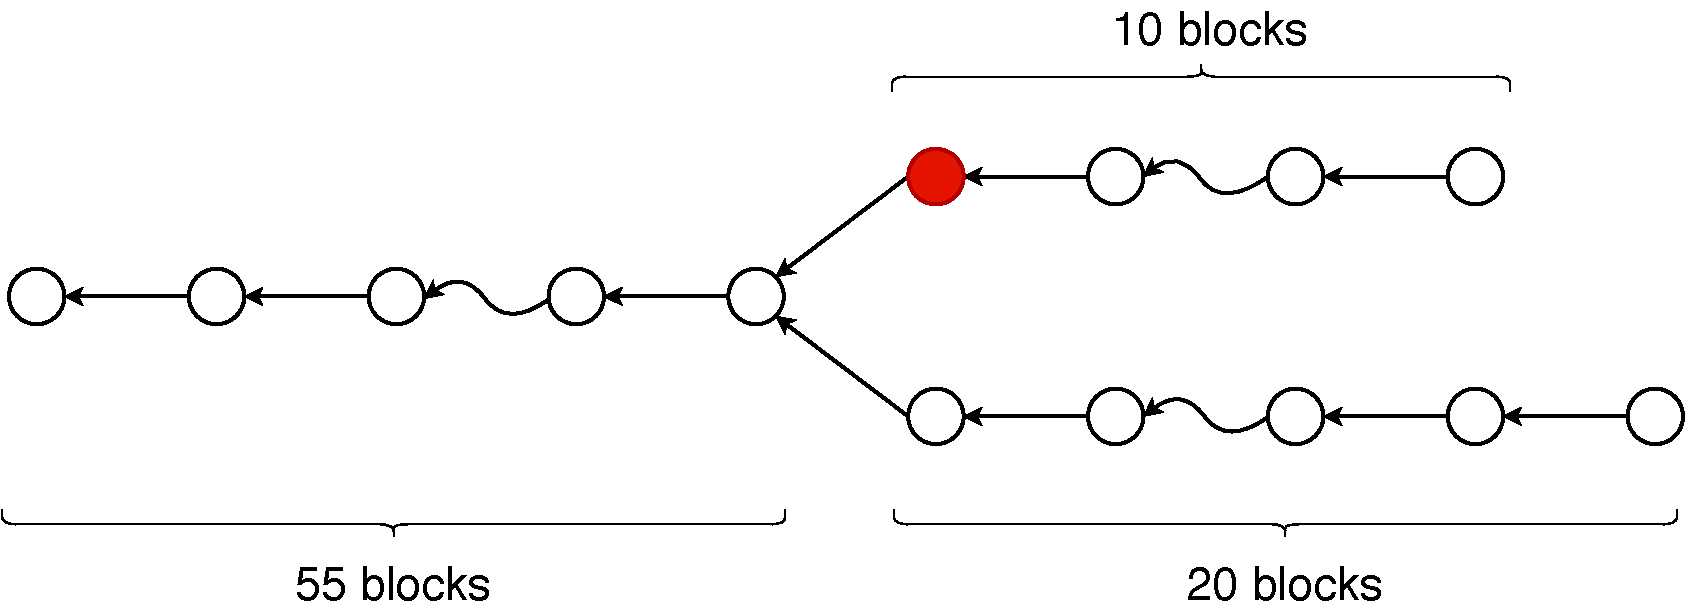
\includegraphics[width=10cm]{./images/proofs_65-10+20.pdf}
    \caption{The red block indicates the block of interest. Curved connections
        imply intermediate blocks. The adversary creates a proof for an event
        that does not exist in the honest chain}
    \label{figure:proofs_65-10+20}
\end{figure}


In this scenario, the original proof is created by an adversary for an event
that does not exist in the honest chain. The proof is contested by an honest
party. We select this configuration because it includes both phases
(submit and contest) and provides full code coverage of each phase since all
underlying operations are executed and no early returns occur.

For a chain of 75 blocks, each phase of the contract needed more than 10
million gas units. Although the size of this test chain is only a very small
faction of the size of a realistic chain, the gas usage already exceeds the
limit of Ethereum blockchain, which is slightly below 10 million. In
particular, the submit of a 650,0000-blocks chain demands 47,280,453 gas. In
Figure \ref{figure:old_gas_per_chain_proof}, we show gas consumption of the submit
phase for different chain sizes and their corresponding proofs sizes. We
demonstrate results for chain sizes from 100 blocks (corresponding to proof size
25) to 650,000 blocks (corresponding to proof size 250).

The linear relation displayed in Figure \ref{figure:old_gas_per_proof} implies
that the gas consumption of the verifier is determined by the size of the
proofs. As shown in Figure \ref{figure:old_gas_per_chain}, the size of the
proofs grows logarithmically to the size of the chain, and this is also
reflected to the gas consumption curve.

\begin{figure}[ht]
\centering
\begin{subfigure}[b]{.49\textwidth}
\begin{tikzpicture}
    \begin{axis}[
        scaled y ticks = true,
        scaled x ticks = false,
        grid=major,
        width=\textwidth,
        xlabel={Chain size},
        ylabel={Gas consumption}
        ]
    \addplot table [col sep=comma] {data/old_gas_per_chain.csv};
\end{axis}
\end{tikzpicture}
\centering
\caption{Gas consumption per chain size}
\label{figure:old_gas_per_chain}
\end{subfigure}
\begin{subfigure}[b]{.49\textwidth}
\begin{tikzpicture}
    \begin{axis}[
        scaled y ticks = true,
        scaled x ticks = false,
        grid=major,
        width=\textwidth,
        xlabel={Proof size},
        ylabel={Gas consumption}
        ]
    \addplot table [col sep=comma] {data/old_gas_per_proof.csv};
\end{axis}
\end{tikzpicture}
\centering
\caption{Gas consumption per proof size}
\label{figure:old_gas_per_proof}
\end{subfigure}
\caption{Gas consumption with respect to chain and corresponding proof size}
\label{figure:old_gas_per_chain_proof}
\end{figure}



\paragraph{Pricing}

So far, we have shown that the verifier is not applicable to the real
blockchain due to extensive gas usage, exceeding the build-in limitation the
Ethereum blockchain by far. While Ethereum adapts to community demands and
build-in parameters can change, it seem improbable to ever incorporate such a
high block gas limit. However, even in this extreme case, the verifier would
still be impractical due to the high cost of the operations in fiat. We call
this amount \emph{toll}, because it is the cost of using the ``bridge'' between
two blockchains. We list these tolls in Table \ref{table:old_cost_in_fiat}. For
this price, we used gas price equal to 5 Gwei, which is considered a
particularly low amount to complete transactions. With this gas price, the
probability approximately that the transaction will be included in one of the
next 200 blocks is 33\%. Note that low and average gas price will not be
sufficient for contesting phase, and it has to be performed with higher gas
price because of the limited contesting period. We will later analyze
thoroughly the entire spectrum of gas prices and tolls for realistic usage of
both submit and contest phases.

\begin{wraptable}{h}{6.0cm}
    \centering
    \begin{tabular}{@{}lccll@{}}
        \toprule
        \multicolumn{1}{c}{\textbf{Chain size}} & \textbf{Toll}  \\ \midrule
        \multicolumn{1}{r}{    100} & \multicolumn{1}{r}{ 12.43 \euro{} } \\
        \multicolumn{1}{r}{    500} & \multicolumn{1}{r}{ 16.14 \euro{} } \\
        \multicolumn{1}{r}{  1,000} & \multicolumn{1}{r}{ 23.79 \euro{} } \\
        \multicolumn{1}{r}{ 10,000} & \multicolumn{1}{r}{ 33.47 \euro{} } \\
        \multicolumn{1}{r}{ 50,000} & \multicolumn{1}{r}{ 44.03 \euro{} } \\
        \multicolumn{1}{r}{100,000} & \multicolumn{1}{r}{ 45.65 \euro{} } \\
        \multicolumn{1}{r}{500,000} & \multicolumn{1}{r}{ 49.88 \euro{} } \\
        \bottomrule
    \end{tabular}
    \caption{Tolls for different chain sizes. Gas price is Gwei}
    \label{table:old_cost_in_fiat}
\end{wraptable}


\subsection{Security Analysis}

We observed that previous work is vulnerable to \emph{premining attack}. We now
lay out an attack, and show how our work mitigates the threat.
\subsubsection{Premining} Premining is the creation of a number of
cryptocurrency coins before the cryptocurrency is launched to the public. There
are altcoins that are based on premining such as AuroraCoin~\cite{aurora}.
Bitcoin, however, is \emph{not} a premined cryptocurrency, since it is proven
that the genesis was created after 3/Jan/2009. In a blockchain where such a
guarantee did not exist, the creator of the chain could quietly mine blocks for
a long time before initiating the public network as displayed in
Figure~\ref{figure:premining_attack}. An adversary could then publish the
private, longer chain, invalidating the public chain which is adopted by the
honest users and hosts all their funds.

\begin{figure}[hbt] \centering

    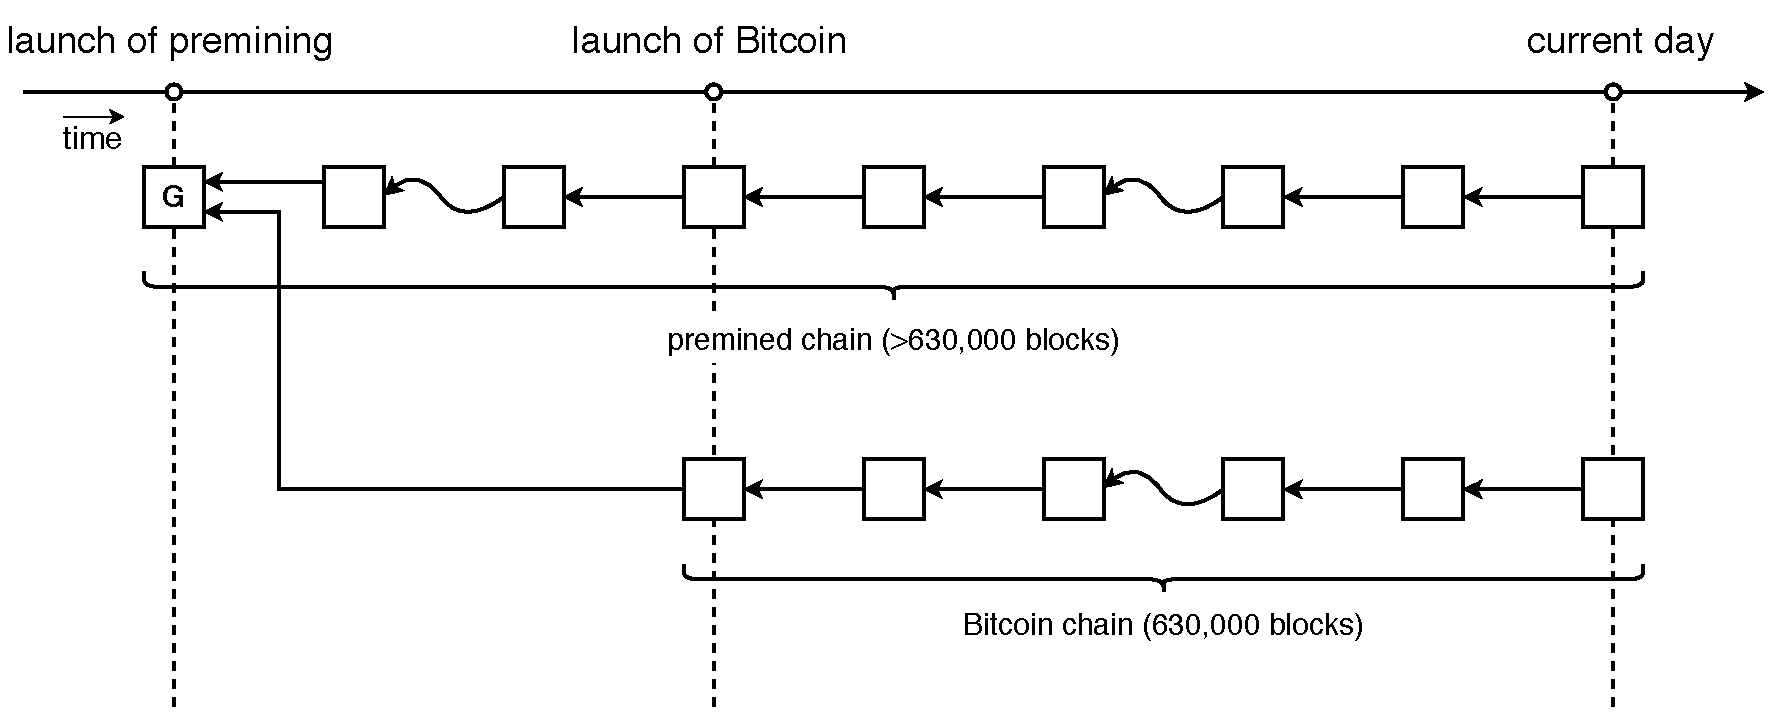
\includegraphics[width=12cm]{./images/premining_attack_bitcoin.pdf}

    \caption{ A premined chain started before the initiation of the public
    network. The older chain contains more blocks and proof-of-work.}

    \label{figure:premining_attack} \end{figure}



The NIPoPoW protocol takes into consideration the $genesis$ block of the
underlying blockchain. We remind that the first block of the chain is always
included in the NIPoPoW by construction. In the NIPoPoW protocol a proof is
structurally correct if two properties are satisfied:

\begin{enumerate}[(a)]

\item The \emph{interlink} structure of all proof blocks is valid.

\item The first block of a proof for a chain $\chain$ is the first block
    $\chain$, the \emph{genesis} block.

\end{enumerate}

From property (b) of NIPoPoWs, we derive that the protocol is resilient to
premining because any chain that does not start from Bitcoin's $genesis$ block,
$\genesis$, results to a proof that also does not start from $\genesis$. Premined
chains start with blocks different than $\genesis$, hence proofs that describe
premined chains are invalid by definition.

\subsubsection{An attack} Previous implementation does require the existence of
underlying chain's $genesis$, exposing the verifier to premining attacks. Such
an attack can be launched by an adversary that mines new blocks on a chain
$\chain_p$ which is prior to the Bitcoin chain $\chain$ as displayed
in~\ref{figure:premining_attack_nipopow}.
\begin{figure}[hbt] \centering

    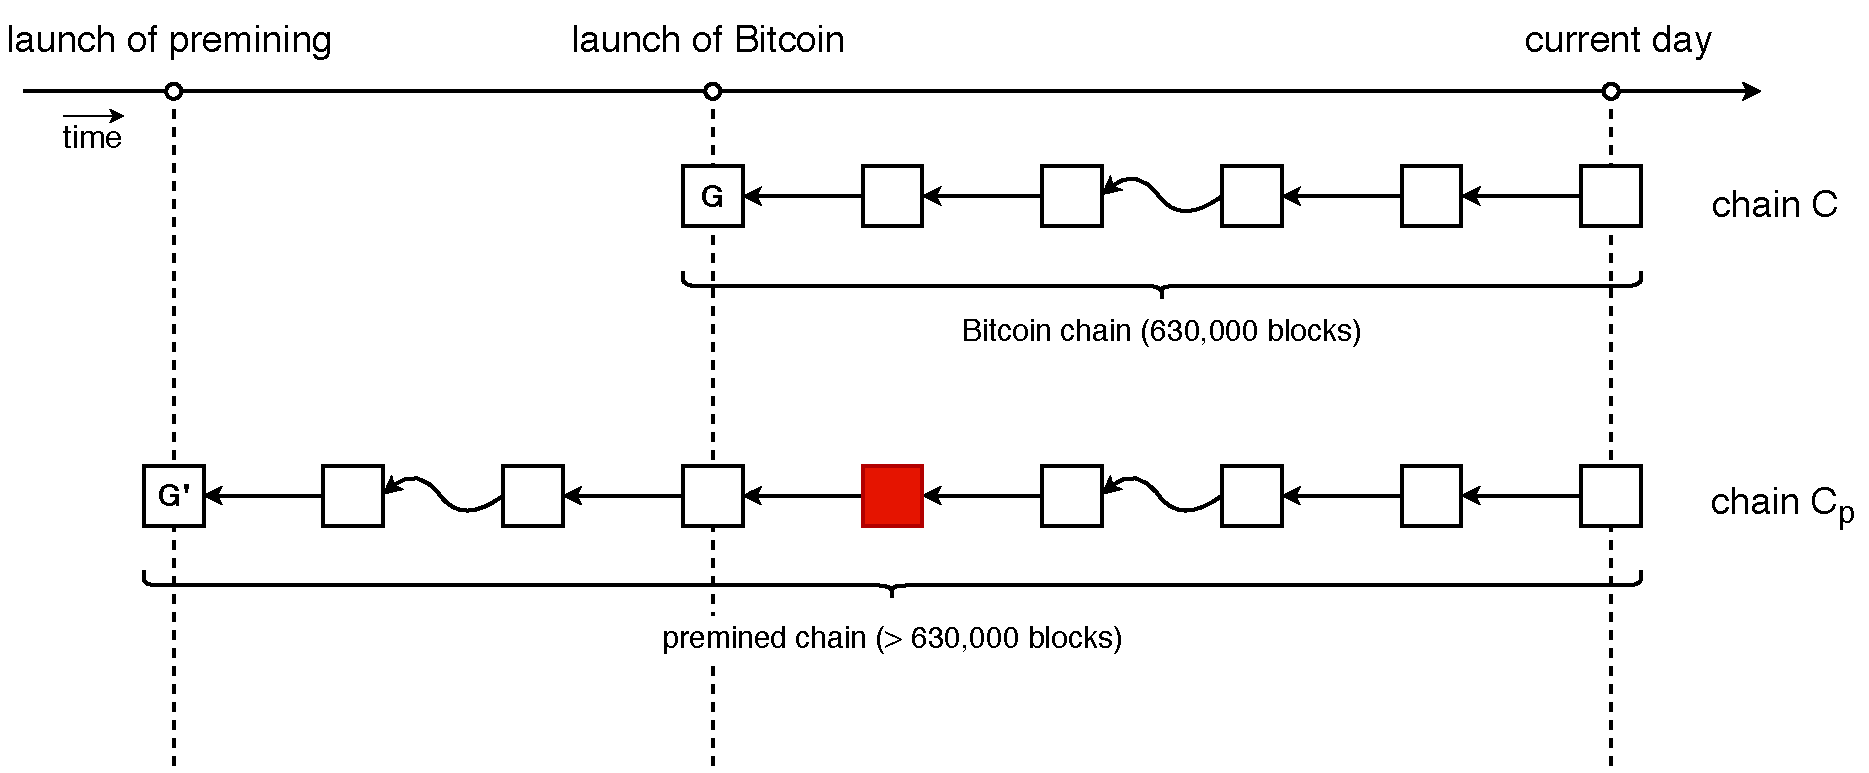
\includegraphics[width=12cm]{./images/premining_attack_nipopow.pdf}

    \caption{ A premined chain started before Bitcoin. The older chain contains
    more blocks.}

    \label{figure:premining_attack_nipopow} \end{figure}


Proofs for events in $\chain_p$ cannot be contested by an honest party, since
chain $\chain_p$ includes more proof-of-work than $\chain$, and thus proofs
with higher score can be generated.

\subsubsection{Mitigation}

We can mitigate this vulnerability by initializing the smart contract with the
$genesis$ block of the underlying blockchain (in our case, Bitcoin) persisting
$genesis$ in storage. For every phase, we add an assertion that the first block
of the proof must be equal to $genesis$. The needed changes are shown in
Algorithm~\ref{alg:avoid-premining}.

These operation do not affect the cost of the verifier because the extra data
saved in storage is constant and small in size (32 bytes).

\begin{algorithm}[H]

    \caption{\label{alg:avoid-premining}The \textsf{NIPoPoW} client mitigation
    to premining attack}
    \begin{algorithmic}[1]

    \Contract{crosschain}
    \State $\textsf{events} \gets \bot$; $\genesis \gets \bot$
    \State $\textsf{DAG} \gets \bot$; $\textsf{ancestors} \gets \bot$
    \Function{\sf initialize}{$\genesis_{remote}$}
        \State $\genesis$ $\gets \genesis_{remote}$
        \Comment{initialize with the genesis of the underlying chain}
    \EndFunction
    \Function{\sf submit}{$\pis$, $e$}
        \State \textsf{require}($\pis$[0] = $\genesis$)
        \Comment{assert correct genesis}
        \State \textsf{require}($\textsf{events$[e]$} = \bot$)
        \State \textsf{require}($\textsf{valid-interlinks}(\pi)$)
        \State \textsf{events$[e].\pi$} $\gets$ $\pis$
        \State \textsf{DAG} $\gets$ \textsf{DAG} $\cup$ $\pi$
        \State \textsf{ancestors} $\gets$ \textsf{find-ancestors(DAG, $\pi$[-1])}
        \State \textsf{require}(\textsf{evaluate-predicate}(\textsf{ancestors}, e))
        \State \textsf{ancestors} $=$ $\bot$
        \EndFunction
    \Function{\sf contest}{$\pic$, $e$}
        \State \textsf{require}($\pic$[0] = $\genesis$)
        \Comment{assert correct genesis}
        \State \textsf{require}(\textsf{events}$[e]$ $\ne$ $\bot$)
        \State \textsf{require}(\textsf{valid-interlinks}($\pic$))
        \State $lca$ = \textsf{find-lca}($\textsf{events}[e].\pi$, $\pic$)
        \State \textsf{require}($\pic$ $\geq_m$ $\textsf{events}[e].\pi$)
        \State \textsf{DAG} $\gets$ \textsf{DAG} $\cup$ $\pic$
        \State \textsf{ancestors} $\gets$
        \textsf{find-ancestors}($\textsf{DAG}$, $\textsf{events}[e].\pi$[-1])
        \State \textsf{require}($\neg$\textsf{evaluate-predicate}(\textsf{ancestors}, $e$))
        \State \textsf{ancestors} $=$ $\bot$
        \State \textsf{events$[e]$} $\gets$ $\bot$
    \EndFunction
    \EndContract
    \vskip8pt
    \end{algorithmic}
\end{algorithm}


